\chapter{Ecuaciones de Maxwell, covariancia y ondas electromagnéticas}

\lectureoverview{Los campos eléctrico y magnético actúan sobre la materia cargada mediante la fuerza de Lorentz, pero la materia también debe crear y reorganizar los campos. Formularemos esa otra mitad recíproca del electromagnetismo, mostraremos que las ecuaciones de Maxwell son covariantes de Lorentz, deduciremos sus soluciones ondulatorias y, después, reincorporaremos la carga y la corriente en una forma que haga manifiesta la conservación local. A lo largo de la lección usaremos unidades en las que \(c=1\).}

\section{La otra mitad del electromagnetismo}

Empecemos por la parte del tema que ya conocemos. Si una partícula de carga \(q\) se mueve con velocidad \(\mathbf v\) a través de campos eléctricos y magnéticos, la fuerza es
\begin{equation}
\mathbf F=q\bigl(\mathbf E+\mathbf v\times\mathbf B\bigr).
\label{eq:lorentz-force-three}
\end{equation}
El factor \(q\) es indispensable. Una partícula sin carga no siente la fuerza electromagnética. El campo eléctrico contribuye incluso cuando la partícula está instantáneamente en reposo, mientras que la contribución magnética depende de su movimiento.

La ecuación~\eqref{eq:lorentz-force-three} nos dice qué efecto tienen sobre la materia unos campos dados. No nos dice qué determina esos campos. ¿Qué produce un campo eléctrico alrededor de un objeto, un campo magnético alrededor de otro o una onda que se propaga por el espacio vacío? Las ecuaciones que responden a esas preguntas son las ecuaciones de Maxwell.

\begin{figure}[H]
\centering
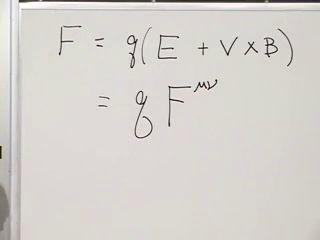
\includegraphics[width=0.62\textwidth]{lecture_58_figure_02.png}
\caption{La fuerza de Lorentz en forma de vector tridimensional y el comienzo de su reformulación tensorial.}
\lectureframe{00:05:49}
\end{figure}

La forma relativista de la ley de fuerza anticipa la notación que necesitaremos:
\begin{equation}
f^\mu=qF^\mu{}_{\nu}u^\nu.
\label{eq:lorentz-force-four}
\end{equation}
Aquí \(u^\nu\) es la cuadrivelocidad, \(f^\mu\) es la cuad fuerza y \(F^{\mu\nu}\) es un tensor antisimétrico construido a partir de \(\mathbf E\) y \(\mathbf B\). En la pizarra se muestra primero solo el comienzo esquemático de esta expresión; la contracción con \(u^\nu\) aporta el vector que falta para dejar un índice de fuerza libre.

Hay una razón física por la que la materia debe actuar también sobre el campo. Una onda electromagnética puede incidir sobre una carga, acelerarla y transferirle energía. Si el campo pudiera afectar a la carga, pero esta nunca pudiera afectar al campo, no habría ningún lugar del que pudiera provenir esa energía. La acción y la reacción no explican por sí solas todo el argumento, pero la conservación de la energía hace inevitable el acoplamiento recíproco.

\section{Una fuente cambiante emite una perturbación}

Una carga puntual produce un campo eléctrico dirigido hacia fuera o hacia dentro desde su posición. Una corriente en un hilo--un flujo de partículas cargadas--produce un campo magnético que circula alrededor del hilo. Estas conocidas imágenes estáticas muestran ya dos patrones geométricos distintos: el flujo eléctrico emana de la carga, mientras que las líneas del campo magnético rodean la corriente.

Ahora desplacemos bruscamente la carga puntual. Cerca de su nueva posición, el campo eléctrico debe empezar a reorganizarse, pero un observador lejano no puede enterarse del movimiento de manera instantánea. El campo antiguo persiste a gran distancia hasta que la señal tiene tiempo de llegar. Entre las regiones cercana y lejana hay un frente en movimiento donde el campo está cambiando. Esa reorganización en movimiento es una perturbación electromagnética.

Si la carga oscila de un lado a otro, las reorganizaciones sucesivas se siguen unas a otras y forman una onda electromagnética. Esta es la función básica de una antena: una corriente eléctrica oscilante envía hacia el exterior una perturbación del campo. Invertir una corriente en un hilo da la versión magnética del mismo argumento. La circulación de \(\mathbf B\) debe invertirse, pero la inversión se propaga en lugar de aparecer simultáneamente en todas partes.

Esta imagen causal fija dos objetivos para las ecuaciones de Maxwell. Deben describir cómo la carga y la corriente generan los campos y permitir que los cambios de esos campos se propaguen a una velocidad que no supere la de la luz. El segundo objetivo también pone a prueba la relatividad. Si las ecuaciones de Maxwell tienen la misma forma en todos los sistemas de referencia inerciales e implican una velocidad de onda definida, todos los observadores inerciales deben deducir de ellas la misma velocidad.

\section{Repaso de la ecuación de ondas relativista}

Antes de pasar a los campos vectoriales, consideremos un campo escalar \(\phi(\mathbf x,t)\), que asigna un número a cada punto del espacio-tiempo. Una ecuación con una derivada,
\begin{equation}
\partial_\mu\phi=0
\end{equation}
indicaría que todas las derivadas respecto del espacio-tiempo se anulan. El campo sería constante y, por tanto, no podría transportar una onda. Una ecuación de ondas relativista no trivial contiene dos derivadas:
\begin{equation}
\partial_\mu\partial^\mu\phi=0.
\end{equation}
Con la convención de signos que usamos aquí,
\begin{equation}
\left(\partial_t^2-\partial_x^2-\partial_y^2-\partial_z^2\right)\phi=0,
\label{eq:scalar-wave-four}
\end{equation}
o, de forma más compacta,
\begin{equation}
\left(\partial_t^2-\nabla^2\right)\phi=0.
\end{equation}
La elección \(c=1\) permite que el tiempo y la distancia tengan unidades compatibles. Al restablecer las unidades habituales, aparecería \(1/c^2\) junto a la segunda derivada temporal.

Para una onda que se propaga a lo largo del eje \(z\), el campo depende de \(z\) y \(t\), pero no de \(x\) ni de \(y\). La ecuación~\eqref{eq:scalar-wave-four} se reduce a
\begin{equation}
\left(\partial_t^2-\partial_z^2\right)\phi=0.
\label{eq:scalar-wave-one}
\end{equation}

\begin{figure}[H]
\centering
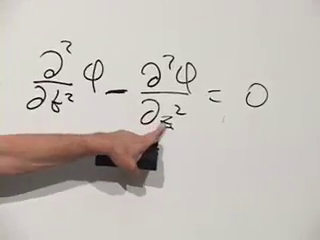
\includegraphics[width=0.56\textwidth]{lecture_58_figure_04.png}
\caption{La ecuación de ondas escalar unidimensional, usada como modelo para las ondas electromagnéticas.}
\lectureframe{00:47:03}
\end{figure}

Su forma general como onda viajera es
\begin{equation}
\phi(z,t)=f(z-t)+g(z+t).
\end{equation}
El perfil \(f(z-t)\) se desplaza hacia valores crecientes de \(z\), ya que un punto de fase constante satisface \(z-t=\text{constant}\). El perfil \(g(z+t)\) se desplaza en sentido contrario. Ninguno de los perfiles tiene por qué ser sinusoidal: cualquier forma suficientemente suave se traslada sin cambiar de forma.

Sin embargo, las funciones sinusoidales son prácticas:
\begin{equation}
\phi(z,t)=A\cos\!\bigl(k(z-t)\bigr).
\end{equation}
El número de onda \(k\) determina la longitud de onda,
\begin{equation}
\lambda=\frac{2\pi}{k}.
\end{equation}
Un valor grande de \(k\) produce oscilaciones espaciales rápidas y una longitud de onda corta; un valor pequeño de \(k\) produce una longitud de onda larga. Pronto, estos mismos perfiles pasarán a ser componentes de \(\mathbf E\) y \(\mathbf B\).

\section{El cálculo vectorial que necesita Maxwell}

Las ecuaciones de Maxwell se expresan mediante productos escalares, productos vectoriales, divergencias y rotacionales. Conviene repasar una vez esta notación, porque en los cálculos por componentes que siguen se usan exactamente estos patrones.

Para los vectores tridimensionales ordinarios \(\mathbf a\) y \(\mathbf b\), el producto escalar es el escalar
\begin{equation}
\mathbf a\cdot\mathbf b
=a_xb_x+a_yb_y+a_zb_z.
\end{equation}
El producto vectorial es otro vector,
\begin{align}
(\mathbf a\times\mathbf b)_x&=a_yb_z-a_zb_y,\\
(\mathbf a\times\mathbf b)_y&=a_zb_x-a_xb_z,\\
(\mathbf a\times\mathbf b)_z&=a_xb_y-a_yb_x.
\end{align}
Las demás componentes se obtienen siguiendo el orden cíclico \(x\to y\to z\to x\).

Introduzcamos el operador diferencial
\begin{equation}
\boldsymbol\nabla=
\left(\partial_x,\partial_y,\partial_z\right).
\end{equation}
Sus componentes son operadores y no números ordinarios, pero aun así pueden aplicarse los patrones del producto escalar y del producto vectorial. Para un campo vectorial \(\mathbf A\),
\begin{equation}
\boldsymbol\nabla\cdot\mathbf A
=\partial_xA_x+\partial_yA_y+\partial_zA_z
\label{eq:divergence}
\end{equation}
es la divergencia, mientras que
\begin{align}
(\boldsymbol\nabla\times\mathbf A)_x
 &=\partial_yA_z-\partial_zA_y,\\
(\boldsymbol\nabla\times\mathbf A)_y
 &=\partial_zA_x-\partial_xA_z,\\
(\boldsymbol\nabla\times\mathbf A)_z
 &=\partial_xA_y-\partial_yA_x
\label{eq:curl}
\end{align}
son las componentes del rotacional.

La geometría es tan importante como las fórmulas. Un campo vectorial tiene divergencia positiva donde parece fluir hacia fuera desde una fuente. Tiene rotacional donde circula. El campo eléctrico radial de una carga puntual ilustra la divergencia; el campo magnético que rodea un hilo por el que circula corriente ilustra el rotacional. Un campo vectorial espacialmente constante no tiene ninguno de los dos.

\section{Las ecuaciones de Maxwell en el vacío}

En ausencia de carga y corriente, las ecuaciones de Maxwell son
\begin{align}
\boldsymbol\nabla\times\mathbf E&=-\partial_t\mathbf B,
\label{eq:faraday-vac}\\
\boldsymbol\nabla\cdot\mathbf B&=0,
\label{eq:gauss-b-vac}\\
\boldsymbol\nabla\times\mathbf B&=\partial_t\mathbf E,
\label{eq:ampere-vac}\\
\boldsymbol\nabla\cdot\mathbf E&=0.
\label{eq:gauss-e-vac}
\end{align}
Las dos ecuaciones del rotacional casi intercambian \(\mathbf E\) y \(\mathbf B\), pero las distingue un signo menos esencial. Las dos ecuaciones de la divergencia indican que ninguno de los campos tiene fuentes en la región de vacío considerada. La divergencia magnética sigue siendo nula incluso cuando se reincorporan las fuentes eléctricas: el electromagnetismo ordinario no contiene carga magnética.

\begin{figure}[H]
\centering
\includegraphics[width=0.76\textwidth]{lecture_58_figure_06.png}
\caption{Las cuatro ecuaciones de Maxwell en el vacío, dispuestas para mostrar la simetría aproximada entre los campos eléctrico y magnético.}
\lectureframe{00:27:30}
\end{figure}

La densidad de carga \(\rho\) acabará sustituyendo al cero en el lado derecho de la ecuación~\eqref{eq:gauss-e-vac}, y la densidad de corriente \(\mathbf J\) aparecerá en la ecuación~\eqref{eq:ampere-vac}. Por ahora, dejamos esos términos de lado. Las ecuaciones sin fuentes ponen de manifiesto la estructura de transformación y el mecanismo de las ondas con el menor número de elementos que distraigan.

También agudizan el enigma de Einstein. Un observador galileano que siguiera una onda esperaría restar velocidades y medir una velocidad de onda menor. Sin embargo, si las mismas ecuaciones de Maxwell son válidas en todos los sistemas inerciales, cada observador deduce la misma velocidad de onda unitaria. La solución no consiste en modificar la ecuación de ondas de un sistema de referencia a otro. Consiste en usar la transformación de Lorentz y expresar las ecuaciones de Maxwell mediante objetos cuyas leyes de transformación ya conocemos.

\section{Los campos eléctrico y magnético como un solo tensor}

Los campos eléctrico y magnético se combinan en el tensor de campo antisimétrico
\begin{equation}
F^{\mu\nu}=
\begin{pmatrix}
0   & -E_x & -E_y & -E_z\\
E_x & 0    & -B_z & B_y\\
E_y & B_z  & 0    & -B_x\\
E_z & -B_y & B_x  & 0
\end{pmatrix},
\label{eq:l0203-field-tensor}
\end{equation}
donde el orden de filas y columnas es \(t,x,y,z\). La antisimetría,
\begin{equation}
F^{\mu\nu}=-F^{\nu\mu},
\end{equation}
obliga a que las entradas diagonales se anulen y determina la mitad inferior de la matriz a partir de la mitad superior. Las entradas espacio-temporales contienen \(\mathbf E\); las entradas puramente espaciales contienen \(\mathbf B\).

\begin{figure}[H]
\centering
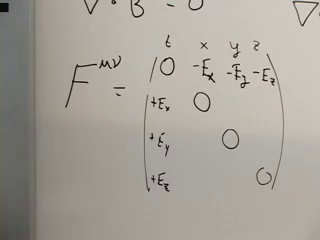
\includegraphics[width=0.58\textwidth]{lecture_58_figure_03.png}
\caption{El tensor de campo electromagnético completo, con sus componentes eléctricas y magnéticas.}
\lectureframe{00:32:05}
\end{figure}

La importancia de \(F^{\mu\nu}\) no reside solo en que sus seis componentes de campo quepan en una matriz. Se transforma como un tensor de rango dos bajo una transformación de Lorentz. Por tanto, los campos eléctrico y magnético que miden distintos observadores se mezclan exactamente de la manera necesaria para que el objeto completo se transforme de forma coherente.

Hay un segundo tensor antisimétrico: el tensor de campo dual \(\widetilde F^{\mu\nu}\). Con la convención actual, se obtiene de la ecuación~\eqref{eq:l0203-field-tensor} mediante el reemplazo
\begin{equation}
\mathbf E\longmapsto-\mathbf B,
\qquad
\mathbf B\longmapsto\mathbf E.
\label{eq:dual-replacement}
\end{equation}
Así,
\begin{equation}
\widetilde F^{\mu\nu}=
\begin{pmatrix}
0    & B_x  & B_y  & B_z\\
-B_x & 0    & -E_z & E_y\\
-B_y & E_z  & 0    & -E_x\\
-B_z & -E_y & E_x  & 0
\end{pmatrix}.
\label{eq:dual-tensor}
\end{equation}
El signo de la ecuación~\eqref{eq:dual-replacement} es importante. Primero, en la lección se intenta expresar verbalmente el intercambio, se detecta la discrepancia de signo y se corrige antes de completar la matriz.

\begin{figure}[H]
\centering
\includegraphics[width=0.58\textwidth]{lecture_58_figure_07.png}
\caption{Construcción del tensor dual mediante el intercambio de las componentes eléctricas y magnéticas con el signo requerido.}
\lectureframe{00:35:45}
\end{figure}

\section{Las ecuaciones covariantes en el vacío}

Cada ecuación de Maxwell contiene una derivada. Si contraemos un tensor de rango dos con una derivada, queda un índice libre, por lo que las opciones covariantes naturales son
\begin{align}
\partial_\mu F^{\mu\nu}&=0,
\label{eq:maxwell-covariant-vac}\\
\partial_\mu\widetilde F^{\mu\nu}&=0.
\label{eq:maxwell-dual-vac}
\end{align}
Para cada valor fijo de \(\nu\), la ecuación~\eqref{eq:maxwell-covariant-vac} es una ecuación. Como \(\nu\) puede tomar los valores \(t,x,y,z\), esta notación reúne cuatro ecuaciones escalares. La ecuación~\eqref{eq:maxwell-dual-vac} reúne las otras cuatro. Esto corresponde a las dos ecuaciones vectoriales del rotacional y a las dos ecuaciones escalares de la divergencia de la lista original.

La notación compacta solo es útil si reproduce las ecuaciones conocidas. Tomemos \(\nu=z\):
\begin{align}
\partial_\mu F^{\mu z}
&=\partial_tF^{tz}
  +\partial_xF^{xz}
  +\partial_yF^{yz}
  +\partial_zF^{zz}\\
&=-\partial_tE_z+\partial_xB_y-\partial_yB_x\\
&=-\partial_tE_z+
  \bigl(\boldsymbol\nabla\times\mathbf B\bigr)_z.
\end{align}
El término \(F^{zz}\) se anula por antisimetría. Al igualar a cero el resultado, obtenemos la componente \(z\) de
\begin{equation}
\boldsymbol\nabla\times\mathbf B=\partial_t\mathbf E.
\end{equation}
Las componentes \(x\) y \(y\) se obtienen mediante permutaciones cíclicas de los índices.

\begin{figure}[H]
\centering
\includegraphics[width=0.76\textwidth]{lecture_58_figure_08.png}
\caption{Desarrollo por componentes de la ecuación covariante de campo: la entrada diagonal del tensor se anula y los términos restantes reconstruyen las ecuaciones de Maxwell.}
\lectureframe{00:43:30}
\end{figure}

Ahora tomemos la componente temporal:
\begin{align}
\partial_\mu F^{\mu t}
&=\partial_tF^{tt}
  +\partial_xF^{xt}
  +\partial_yF^{yt}
  +\partial_zF^{zt}\\
&=\partial_xE_x+\partial_yE_y+\partial_zE_z\\
&=\boldsymbol\nabla\cdot\mathbf E.
\end{align}
Por tanto, da la ecuación~\eqref{eq:gauss-e-vac}. Al hacer las mismas comprobaciones con el tensor dual, se obtienen
\(\boldsymbol\nabla\cdot\mathbf B=0\) y
\(\boldsymbol\nabla\times\mathbf E=-\partial_t\mathbf B\).

Ahora las ecuaciones compactas están demostradas, no solo conjeturadas. Su estructura con índices libres las convierte en ecuaciones de cuadrivectores, de modo que una transformación de Lorentz cambia sus componentes, pero no su forma. Este es el sentido preciso en que las ecuaciones de Maxwell en el vacío son iguales en todos los sistemas de referencia inerciales.

\section{De las ecuaciones de primer orden a una onda}

Las ecuaciones de Maxwell contienen solo derivadas de primer orden, mientras que una ecuación de ondas contiene derivadas de segundo orden. La aparente discrepancia se resuelve porque la teoría de Maxwell acopla dos campos. Un par de ecuaciones de primer orden para \(\mathbf E\) y \(\mathbf B\) puede combinarse para obtener una ecuación de segundo orden para cualquiera de los dos campos por separado.

Derivemos la ecuación~\eqref{eq:ampere-vac} respecto del tiempo:
\begin{equation}
\partial_t^2\mathbf E
=\boldsymbol\nabla\times\partial_t\mathbf B.
\end{equation}
La ley de Faraday proporciona la derivada temporal de \(\mathbf B\):
\begin{equation}
\partial_t\mathbf B=-\boldsymbol\nabla\times\mathbf E,
\end{equation}
y, por tanto,
\begin{equation}
\partial_t^2\mathbf E
=-\boldsymbol\nabla\times
  \bigl(\boldsymbol\nabla\times\mathbf E\bigr).
\label{eq:double-curl}
\end{equation}

En la pizarra se desarrolla una componente en lugar de recurrir a una identidad memorizada. Para la componente \(x\),
\begin{align}
\bigl[\boldsymbol\nabla\times
(\boldsymbol\nabla\times\mathbf E)\bigr]_x
&=\partial_y(\boldsymbol\nabla\times\mathbf E)_z
 -\partial_z(\boldsymbol\nabla\times\mathbf E)_y\\
&=\partial_y(\partial_xE_y-\partial_yE_x)\\
&\quad-\partial_z(\partial_zE_x-\partial_xE_z)\\
&=\partial_x(\partial_yE_y+\partial_zE_z)
 -\partial_y^2E_x\\
&\quad-\partial_z^2E_x.
\end{align}
Sumemos y restemos \(\partial_x^2E_x\) para poner de manifiesto la divergencia:
\begin{align}
\bigl[\boldsymbol\nabla\times
(\boldsymbol\nabla\times\mathbf E)\bigr]_x
&=\partial_x(\boldsymbol\nabla\cdot\mathbf E)
 -\nabla^2E_x.
\label{eq:double-curl-x}
\end{align}
En el vacío, \(\boldsymbol\nabla\cdot\mathbf E=0\). Al combinar las ecuaciones~\eqref{eq:double-curl} y \eqref{eq:double-curl-x}, obtenemos
\begin{equation}
\left(\partial_t^2-\nabla^2\right)E_x=0.
\label{eq:ex-wave}
\end{equation}

\begin{figure}[H]
\centering
\includegraphics[width=0.72\textwidth]{lecture_58_figure_09.png}
\caption{El cálculo por componentes llega a la ecuación de ondas para \(E_x\).}
\lectureframe{00:57:10}
\end{figure}

El mismo cálculo se aplica a \(E_y\) y \(E_z\), y una eliminación análoga da
\begin{equation}
\left(\partial_t^2-\nabla^2\right)\mathbf B=0.
\end{equation}
Por tanto, los campos eléctrico y magnético pueden propagarse como ondas por el espacio vacío. En las unidades que usamos, su velocidad es uno; al restablecer las unidades habituales, esto significa que la velocidad es \(c\).

\section{Una onda plana y su polarización}

Construyamos una onda sencilla que se propague en la dirección positiva de \(z\):
\begin{equation}
\mathbf E(z,t)
=\widehat{\mathbf x}\,E_0
  \cos\!\bigl(k(z-t)\bigr).
\label{eq:plane-e}
\end{equation}
Su perfil se traslada a lo largo de \(z\) sin cambiar de forma. Como el campo eléctrico apunta a lo largo del eje \(x\), la onda está polarizada linealmente en la dirección \(x\). Hemos elegido \(E_y=0\) solo para mantener sencillo el ejemplo; podría incluirse una segunda polarización transversal.

La componente longitudinal no es igual de libre. Como la onda depende solo de \(z\) y \(t\),
\begin{equation}
\boldsymbol\nabla\cdot\mathbf E
=\partial_zE_z=0.
\end{equation}
Así, \(E_z\) puede ser constante, pero no puede contener el perfil ondulatorio variable. Puede superponerse o eliminarse por separado un campo de fondo uniforme; este no forma parte de la radiación que se propaga. La onda en sí es transversal:
\begin{equation}
\mathbf E_{\mathrm{wave}}\cdot\widehat{\mathbf z}=0.
\end{equation}

La ley de Faraday determina el campo magnético. Para la ecuación~\eqref{eq:plane-e}, la única componente no nula de \(\boldsymbol\nabla\times\mathbf E\) es la componente \(y\):
\begin{equation}
(\boldsymbol\nabla\times\mathbf E)_y=\partial_zE_x.
\end{equation}
En consecuencia, \(\partial_t\mathbf B\) apunta en la dirección \(y\), y una elección compatible es
\begin{equation}
\mathbf B(z,t)
=\widehat{\mathbf y}\,E_0
  \cos\!\bigl(k(z-t)\bigr).
\label{eq:plane-b}
\end{equation}
En estas unidades, las amplitudes eléctrica y magnética son iguales. Su orientación satisface
\begin{equation}
\mathbf E\perp\mathbf B,
\qquad
\mathbf E\perp\widehat{\mathbf z},
\qquad
\mathbf B\perp\widehat{\mathbf z},
\qquad
\mathbf E\times\mathbf B\parallel\widehat{\mathbf z}.
\end{equation}

\begin{figure}[H]
\centering
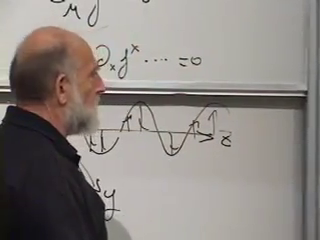
\includegraphics[width=0.70\textwidth]{lecture_58_figure_05.png}
\caption{Esquema completo de la pizarra de una onda electromagnética transversal: las oscilaciones de los campos eléctrico y magnético son perpendiculares entre sí y a la dirección de propagación.}
\lectureframe{01:05:25}
\end{figure}

\begin{figure}[H]
\centering
\scalebox{0.90}{%
\begin{tikzpicture}[x=1cm,y=1cm,>=Latex]
  \draw[->,thick] (0,0) -- (8.2,0) node[right] {$z$};
  \draw[->,thick] (0,-1.6) -- (0,1.7) node[above] {$x$};
  \draw[->,thick] (0,0) -- (-1.15,-0.8) node[below left] {$y$};
  \draw[blue!70!black,thick,domain=0:7.5,samples=120]
    plot (\x,{0.95*sin(90*\x)});
  \foreach \z/\s in {0.8/1,2.8/-1,4.8/1,6.8/-1}{
    \draw[->,green!45!black,thick]
      (\z,0) -- ++({-0.55*\s},{-0.38*\s});
  }
  \node[blue!70!black] at (6.9,1.25) {$\mathbf E$};
  \node[green!45!black] at (5.2,-1.05) {$\mathbf B$};
  \draw[->,very thick] (6.2,1.55) -- (7.7,1.55)
    node[midway,above] {propagation};
\end{tikzpicture}
}
\caption{Los campos \(\mathbf E\) y \(\mathbf B\) son perpendiculares entre sí y a la dirección de propagación.}
\end{figure}

Esta es la naturaleza de la luz y de toda radiación electromagnética en el vacío. Como las ecuaciones que producen la onda son covariantes de Lorentz, otro observador inercial describe, a su vez, una onda electromagnética que se propaga a \(c\), con campos eléctrico y magnético transversales.

\section{Densidad de carga y densidad de corriente}

Ahora reincorporamos las fuentes que habíamos dejado temporalmente de lado. Cuando una región contiene muchas partículas cargadas, resulta útil aproximarlas como una densidad de carga continua
\begin{equation}
\rho(\mathbf x,t)=\frac{dQ}{dV}.
\end{equation}
La aproximación es similar a tratar el agua como un fluido continuo, aunque esté formada por moléculas. Las cargas positivas y negativas contribuyen con signos opuestos, por lo que \(\rho\) es la carga neta por unidad de volumen.

La carga en una región elegida \(V\) es
\begin{equation}
Q_V(t)=\int_V\rho(\mathbf x,t)\,dV.
\label{eq:charge-volume}
\end{equation}
La densidad puede variar con la posición y el tiempo. Una acumulación de carga puede alejarse de un punto y cambiar allí la densidad local. Sin embargo, esta no puede variar de forma arbitraria. La naturaleza conserva la carga eléctrica.

La conservación global por sí sola sería demasiado débil. Permitiría que la carga desapareciera de la Tierra y reapareciera en Marte en el mismo instante, siempre que el total no cambiara. La afirmación más fuerte es local: la carga solo puede salir de un lugar y llegar a otro si fluye por el espacio intermedio.

Para describir ese flujo, tomemos un elemento de superficie infinitesimal orientado
\begin{equation}
d\boldsymbol\sigma=\widehat{\mathbf n}\,d\sigma.
\end{equation}
Su módulo es el área y su dirección es normal a la superficie. La densidad de corriente \(\mathbf J\) se define de modo que la carga que atraviesa el elemento por unidad de tiempo sea
\begin{equation}
\frac{dQ}{dt}=\mathbf J\cdot d\boldsymbol\sigma.
\label{eq:current-flux-element}
\end{equation}
El módulo de \(\mathbf J\) es la carga por unidad de área y por unidad de tiempo, y su dirección es la del flujo de carga positiva.

\begin{figure}[H]
\centering
\includegraphics[width=0.64\textwidth]{lecture_58_figure_10.png}
\caption{Un elemento de área orientado y el factor de flujo \(d\boldsymbol\sigma\cdot\mathbf J\).}
\lectureframe{01:18:15}
\end{figure}

El producto escalar selecciona la componente normal a la superficie. Una corriente tangente a la superficie no atraviesa ninguno de sus lados y aporta cero. Una corriente paralela a la normal da el flujo máximo para un módulo fijo. La corriente en un hilo es un caso particular, pero \(\mathbf J\) también puede describir carga que fluye a través de una lámina o por todo el espacio tridimensional.

\section{Conservación local y ecuación de continuidad}

Fijemos una región \(V\) del espacio y orientemos hacia fuera cada elemento de su frontera cerrada \(\partial V\). Si hay una corriente neta saliente, la carga en el interior disminuye:
\begin{equation}
\frac{dQ_V}{dt}
=-\oint_{\partial V}\mathbf J\cdot d\boldsymbol\sigma.
\label{eq:integral-conservation}
\end{equation}
El signo menos tiene un significado físico, no es una convención: el flujo positivo saliente extrae carga positiva de la región. Usando la ecuación~\eqref{eq:charge-volume},
\begin{equation}
\int_V\partial_t\rho\,dV
=-\oint_{\partial V}\mathbf J\cdot d\boldsymbol\sigma.
\label{eq:integral-continuity-one}
\end{equation}

\begin{figure}[H]
\centering
\includegraphics[width=0.72\textwidth]{lecture_58_figure_11.png}
\caption{Ley de conservación para una región fija, una vez convertido el flujo superficial en una expresión de volumen.}
\lectureframe{01:29:00}
\end{figure}

El teorema de Gauss, también llamado teorema de la divergencia, relaciona el flujo a través de una superficie cerrada con la divergencia en su interior:
\begin{equation}
\oint_{\partial V}\mathbf A\cdot d\boldsymbol\sigma
=\int_V\boldsymbol\nabla\cdot\mathbf A\,dV.
\label{eq:divergence-theorem}
\end{equation}
Podemos imaginar tuberías ocultas que inyectan agua en distintos puntos del interior de un recipiente. La divergencia mide la tasa local a la que el agua sale de los extremos de las tuberías; la integral de superficie mide la cantidad total de agua que sale del recipiente. Todo lo que se genera como flujo saliente en el interior debe acabar atravesando la frontera.

Al aplicar la ecuación~\eqref{eq:divergence-theorem} a \(\mathbf J\), obtenemos
\begin{equation}
\int_V
\left(\partial_t\rho+\boldsymbol\nabla\cdot\mathbf J\right)dV=0.
\end{equation}
Esta relación es válida para cualquier región \(V\) posible. Por tanto, el integrando debe anularse punto por punto:
\begin{equation}
\boxed{\partial_t\rho+\boldsymbol\nabla\cdot\mathbf J=0.}
\label{eq:continuity-three}
\end{equation}

\begin{figure}[H]
\centering
\includegraphics[width=0.72\textwidth]{lecture_58_figure_12.png}
\caption{La ecuación de continuidad local escrita componente por componente.}
\lectureframe{01:29:50}
\end{figure}

La ecuación~\eqref{eq:continuity-three} expresa exactamente lo que exige la conservación local. Si la densidad de carga disminuye en un punto o en una región pequeña, la corriente debe divergir hacia fuera de allí. Si la corriente converge hacia dentro, la densidad de carga aumenta.

La densidad y la corriente forman de manera natural la cuadr corriente
\begin{equation}
J^\mu=(\rho,J_x,J_y,J_z)
\label{eq:four-current}
\end{equation}
en unidades \(c=1\). La ecuación de continuidad se convierte en la ecuación escalar de Lorentz
\begin{equation}
\partial_\mu J^\mu=0.
\label{eq:continuity-four}
\end{equation}
El flujo de una distribución relativista debe transformarse como un cuadrivector, igual que la cuadrivelocidad de una partícula. La ecuación~\eqref{eq:continuity-four} hace que la conservación local de la carga sea válida en todos los sistemas de referencia inerciales.

\section{Las ecuaciones de Maxwell con fuentes}

Al reincorporar la carga y la corriente, obtenemos
\begin{align}
\boldsymbol\nabla\cdot\mathbf E&=\rho,
\label{eq:gauss-e-source}\\
\boldsymbol\nabla\cdot\mathbf B&=0,\\
\boldsymbol\nabla\times\mathbf E&=-\partial_t\mathbf B,\\
\boldsymbol\nabla\times\mathbf B&=\partial_t\mathbf E+\mathbf J.
\label{eq:ampere-source}
\end{align}
Las ecuaciones que incluyen fuentes eléctricas se condensan en
\begin{equation}
\boxed{\partial_\mu F^{\mu\nu}=J^\nu,}
\label{eq:maxwell-source-covariant}
\end{equation}
mientras que el par magnético sin fuentes sigue siendo
\begin{equation}
\boxed{\partial_\mu\widetilde F^{\mu\nu}=0.}
\label{eq:maxwell-dual-source}
\end{equation}

\begin{figure}[H]
\centering
\includegraphics[width=0.78\textwidth]{lecture_58_figure_13.png}
\caption{Las ecuaciones de Maxwell con fuentes, junto a su forma covariante \(\partial_\mu F^{\mu\nu}=J^\nu\).}
\lectureframe{01:34:00}
\end{figure}

La componente temporal de la ecuación~\eqref{eq:maxwell-source-covariant} se escribe
\begin{equation}
\partial_\mu F^{\mu t}=J^t=\rho,
\end{equation}
y el cálculo por componentes que ya realizamos transforma su lado izquierdo en
\(\boldsymbol\nabla\cdot\mathbf E\). Las tres componentes espaciales reproducen
\(\boldsymbol\nabla\times\mathbf B=\partial_t\mathbf E+\mathbf J\).

Hay también una comprobación útil de consistencia. Al aplicar \(\partial_\nu\) a la ecuación~\eqref{eq:maxwell-source-covariant}, obtenemos
\begin{equation}
\partial_\nu J^\nu
=\partial_\nu\partial_\mu F^{\mu\nu}=0,
\end{equation}
porque las dos derivadas son simétricas bajo el intercambio \(\mu\leftrightarrow\nu\), mientras que \(F^{\mu\nu}\) es antisimétrico.\editorialnote{Esta breve comprobación de consistencia se deduce de la ecuación covariante y hace explícito por qué las ecuaciones de Maxwell con fuentes respetan automáticamente la ecuación de continuidad.}

La estructura recíproca ya está completa. La ley tensorial de fuerza
\(f^\mu=qF^\mu{}_\nu u^\nu\)
describe cómo actúan los campos sobre la carga, y la ecuación~\eqref{eq:maxwell-source-covariant} describe cómo la carga y la corriente generan campos. Ambas son ecuaciones tensoriales. En el vacío, las mismas ecuaciones de campo dan lugar a ondas transversales que se propagan a \(c\). Así, la covariancia de Lorentz y la ecuación de ondas electromagnéticas se encuentran en el punto que motivó esta construcción: todos los observadores inerciales obtienen las mismas leyes del electromagnetismo y la misma velocidad de la luz.
